% id: 0700
% book: 라이트쎈 공통수학1 · 05 이차방정식과 이차함수
% section: 서술형
% figure: tikz:fig-0700
% answer: $100\,\mathrm{cm}^2$
% answer_source: 답지
% variant_level: 0 (원본 전사)
% 이 파일은 build.mjs 가 items.json 에서 만든다. 고칠 때는 items.json 을 고친다.
\smash{\raisebox{1.5mm}{\dmkichul{라이트쎈 공통수학1 0700번 · 97쪽}}}
\noindent\begin{minipage}[t]{0.58\linewidth}\vspace{0pt}\raggedright 오른쪽 그림과 같이 가로의 길이가 $12\,\mathrm{cm}$, 세로의 길이가 $8\,\mathrm{cm}$인 직사각형에서 가로의 길이는 $x\,\mathrm{cm}$만큼 줄이고 세로의 길이는 $x\,\mathrm{cm}$만큼 늘여서 새로운 직사각형을 만들려고 한다. 이때 새로운 직사각형의 넓이의 최댓값을 구하시오. \cond{$x>0$}\end{minipage}\hfill\begin{minipage}[t]{0.4\linewidth}\vspace{0pt}\centering \resizebox{\ifdim\width>\linewidth\linewidth\else\width\fi}{!}{% 0700(본책 97쪽) — 가로 12 cm·세로 8 cm 직사각형(윤곽)과, 가로를 x cm 줄이고 세로를 x cm 늘인 새 직사각형(연녹 채움). 라벨은 원문의 12 cm·8 cm·x cm·x cm 뿐. 스캔 그림이라 TikZ 로 다시 그림.
% x 의 크기는 답이 읽히지 않게 임의로 둠.
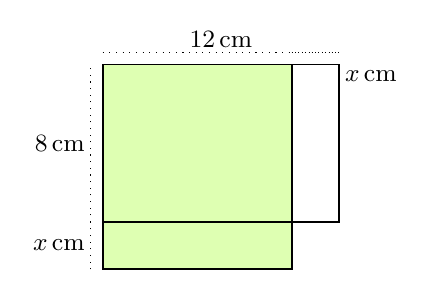
\begin{tikzpicture}[scale=1, line width=0.5pt]
  \fill[green!25!lime!30] (0,-0.6) rectangle (2.4,2);
  \draw[line width=0.6pt] (0,0) rectangle (3,2);
  \draw[line width=0.6pt] (0,-0.6) rectangle (2.4,2);
  \draw[dotted, line width=0.4pt] (0,2.15) -- (3,2.15);
  \draw[dotted, line width=0.4pt] (-0.15,0) -- (-0.15,2);
  \draw[dotted, line width=0.4pt] (-0.15,-0.6) -- (-0.15,0);
  \draw[dotted, line width=0.4pt] (2.4,2.15) -- (3,2.15);
  \node[above, font=\small, inner sep=1.5pt] at (1.5,2.15) {$12\,\mathrm{cm}$};
  \node[left, font=\small, inner sep=2pt] at (-0.15,1) {$8\,\mathrm{cm}$};
  \node[left, font=\small, inner sep=2pt] at (-0.15,-0.3) {$x\,\mathrm{cm}$};
  \node[right, font=\small, inner sep=2pt] at (3,1.85) {$x\,\mathrm{cm}$};
\end{tikzpicture}
}\end{minipage}\par
